\documentclass[a4paper]{article}

\usepackage{xcolor}
\usepackage{fancyhdr}
\usepackage{listings}
\usepackage[dutch]{babel}
\usepackage{graphicx}


\newcommand{\todo}[1]{\textcolor{red}{[#1]}}
\lhead{Open Universiteit}
\chead{IM0102, Design patterns}
\rhead{Final assignment}

\begin{document}
\pagestyle{fancy}

\section*{Student information}
\begin{description}
	\item [Cursuscode] IM0102
	\item [Scenario] JabberPoint with themes
	\item [Name] A. Slomp
	\item [Student number] 838768442
	\item [Name] W. van der Weij
	\item [Student number] 851988675
\end{description}

\section{Introduction}
This is our report of the final assignment of the Design patterns course of the Open Universiteit. In this report we describe our solution to the redesign of the JabberPoint application.

This report is structured as follows.
The report starts with a description of the way we worked together on the assignment. 
The problem analysis describes the goal, concepts with commonality and variability analysis, application functionality and the assumptions during the assignment. \todo{add more structure later}


\section{Project execution}

Here we describe how we handled the assignment together. The numbers indicate the explicit ordering of the activities. 

1. We both studied the assignment separately to prepare for our first meeting. 

2. After a couple of days we met at Wilkos place for the first time to discuss the assignment. Together we went through the assignment, the program code, the running application and we discussed possible solutions on conceptual level as well on implementation level. Just exchanging ideas, brain storming and discussing about possible solutions. We also discussed the tools to use (Eclipse with Papyrus plugin) and the format of the report (Latex).
Furthermore we looked together at the git repository, the usage of github.com and how to operate it locally. We also discussed the planning of the assignment.  

3. We both started working on the assignment separately. We both agreed to do most of the work separately, but based on our discussions and compare solutions. From our discussions we decided to have a different focus, but still do the work both. Arend focusing on the class diagrams already and Wilko focusing on the problem analysis.

4. About a week after the first meeting, we met again to discuss our progress. This time at Arends place. We still had a lot to discuss. We went through the code, annotating it with TODOs at places with strange code or remarkable design. We went through two more documents from you learn: \textit{Guidelines redesign} and \textit{Beoordeling Design patterns}. The work to be done seemed more than the expectations we had after the first meeting. Again we agreed to do both the work with focus on different items. Arend puts together both reports and looks at the design, while Wilko does the CVA, choices and description of design patterns to be used.

5. We both continued work on the assignment separately, but together. Thinking and about the problem analysis and the design, drawing diagrams, looking at code and already cleaning up code. 

6. Three days before the deadline we met again. We discussed our progress and the priorities of the remaining work. 

7. We divided the work again and started polishing things up. We had to put an amount of work to document all the notes and diagrams we had written and drawn during our discussions. Tools to draw UML diagrams are handy and even indispensable, but during discussions and brainstorming a paper and pen are superior.

\section{Problem analysis}
The assignment is to redesign the existing application JabberPoint to support multiple themes. The feature request is to let the user pick one of the available themes and apply the new styles to the content of the presentation. The selected theme should be applied to the current application and the current slide.

Besides the addition of the feature request, the application is redesigned further. The goal is to improve the quality of the application overall and to achieve a better user experience, increased flexibility and easier maintainability.  

Out of scope are at this moment:
\begin{itemize}
\item editing presentations
\item editing themes 
\end{itemize}

\subsection{Application functionality}
The JabberPoint application is started with the internal demo presentation or a presentation loaded from a file specified by the command line parameter. The first slide of the presentation is displayed.
JabberPoint accepts one optional parameter during startup: a presentation file. 
An invalid parameter value results in an application without any presentation loaded.

The view of the application consists of a program window with a menubar at the top. The application is operated by a pointing device and a keyboard. 

Menu items and key assignments:
\begin{itemize}
\item{Open} goal unclear, should let the user open a presentation? 
\item{New} clears the current presentation
\item{Save} saves the presentation (writes theme)
\item{Exit} Exits the application. Key: q or Q
\end{itemize}

Slide actions:
\begin{itemize}
\item{Next slide} show next slide. Keys: \textless page down\textgreater, \textless arrow down\textgreater, \textless enter\textgreater{ }or '+'
\item{Previous slide} show previous slide. Keys: \textless page up\textgreater, \textless arrow up\textgreater{ }or '-'
\item{Goto slide} show the slide with specified number. menu, shortcut
\end{itemize}

Help actions:
\begin{itemize}
\item{About} show a popup with information about JabberPoint.
\end{itemize}

New action:
\begin{itemize}
\item{Select theme} Let the user select a theme. 
\end{itemize}

The presentation content could be read from a file or otherwise a demo presentation from within the application is read

JabberPoint does not support editing of presentations.

\subsection{Concepts}

A \textit{presentation} consists of a number of sequential slides, which a user can step through forward and backwards. The presentation displays information to the audience during a talk or speech. In the context of this document a presentation is the content that the JabberPoint application shows and it is not the speech or talk to an audience itself.
 
A \textit{slide} is a page in a presentation that contains display elements like text and graphics. The display elements are displayed according to predefined styles. Every slide has a title.

A slide contains \textit{item}s such as text and images. All these items have varying and some overlapping  behaviours, such as: font type, text size, background colour and size. The items on a slide have a indentation, which is also related with the appearance or style of the item. 

\textit{Theme}s arange the displaying of the elements of a presentation. A theme consists of styles that control the display behaviour such as background colour, text colour and font size. The styles within the theme are stacked and the levels are leading when a theme is applied to a slide.  

A \textit{style} prescribes the displaying behaviour of items on slides. 

The \textit{view} of the application consists of a window that has a menubar at the top left. The remainder of the window is used to render the slides of a presentation according to the styles that are defined for that side.

The application is able to read a XML file that contains a presentation according to a defined structure.    

\begin{table}[!htpb]
\centering
\begin{tabular}{|l|l|l|l|}
\hline
\textbf{Commonality} & \textbf{Variability} & \textbf{Knows} & \textbf{Can}\\
\hline
\hline
Presentation & One of a kind & Title, theme, slides, current slide & Step through slides.\\
\hline
Slide & One of a kind & Title, items on slide & None\\ 
\hline
Items on slide & Text, image & Level, specific properties & None\\
\hline
Theme & One of a kind & Name, styles and background color & None\\
\hline
Style & One of a kind & Indent, line spacing, font properties & None\\
\hline
\end{tabular}
\caption{Things}
\label{tab:template}
\end{table}

\subsection{Rules}
In the problem domain there are rules the concepts adhere to:
\begin{itemize}
\item{Depending on the startup parameter a demo \textit{presentation} or a presentation read from disk is shown.}
\item{The \textit{level} of a \textit{style} in a \textit{theme} matches the \textit{level} of a n\textit{item} on a \textit{slide}.}
\item{The \textit{items} on a \textit{slide} are displayed from top to bottom.}
\end{itemize}

\subsection{Actions}

\begin{table}[!htpb]
\centering
\begin{tabular}{|l|l|l|l|}
\hline
\textbf{Action} & \textbf{Description}\\
\hline
\hline
Open & Goal within the application unclear, expected to open a \textit{presentation}.\\
\hline
Save & Stores the \textit{presentation} with the currently selected \textit{theme}.\\ 
\hline
Exit & Ends the \textit{application}.\\
\hline
Next & Step to the next \textit{slide} of the \textit{presentation}, if possible.\\
\hline
Previous & Step to the previous \textit{slide} of the \textit{presentation}, if possible.\\
\hline
Go to & Step to a specific \textit{slide} of the \textit{presentation}, if possible.\\
\hline
Select theme & Select a \textit{theme} to apply to the current \textit{presentation}.\\
\hline
Show slide & Draw the current \textit{slide} with \textit{item}s according to the correct \textit{style}s.\\
\hline
\end{tabular}
\caption{Actions}
\label{tab:template}
\end{table}

\subsection{Assumptions}
Assumption is that altering the supported file format is allowed, as long as the application is backwards compatible.

Assumption is that bug fixes are appreciated as long as functionality is not decreased. The behaviour of the next, previous and goto functionality is buggy. Several scenario's result in failures. For example the goto functionality does not validate input, resulting in errors and faulty behaviour for non-numerical and out of range values. Hitting next or previous slide quickly after each other let the presentation disappear (in MacOS with the menu options shortcuts).   

\section{Design for change}
We redesigned the JabberPoint application to handle changes well. We all know changes will come. We tried to accommodate change on all levels from software design and architecture to programming code. In this section we elaborate on these levels.

\subsection{Guidelines and principles} 
Design decisions during the design process are guided by design principles and guidelines that we describe briefly.
We have a couple of design principles:
\begin{itemize}
\item Single responsibility principle. Do one thing and do it well, without side effects. Separated responsibilities lead to high cohesion. A class should be responsible for itself.
\item Open-closed principle. Open for extension, closed for modification. Make future changes without breaking existing classes.
\item Don't repeat yourself principle. There must be a lack of redundancy. Rules should be implemented once. One rule, one place.
\item Liskov substitution principle. Subtypes should be substitutable for base types. Well designed inheritance. 
\end{itemize}

Other guidelines or best practices are:
\begin{itemize}
\item Prefer delegation over inheritance.
\item Program to interfaces or abstract classes.
\item Each interface should have one reason to change.
\end{itemize}
These principles and guidelines should lead to clarity, high cohesion and low coupling. These are ingredients for a flexible and easy to extend application. We think that is exactly what JabberPoint needs to be. 

\subsection{Package structure}
We designed the package structure according to the package-by-layer style (see choices).
The package dependencies are hierarchical and non-circular. In the package diagram one can see all arrows are one way dependencies.

\begin{figure}[!htpb]
  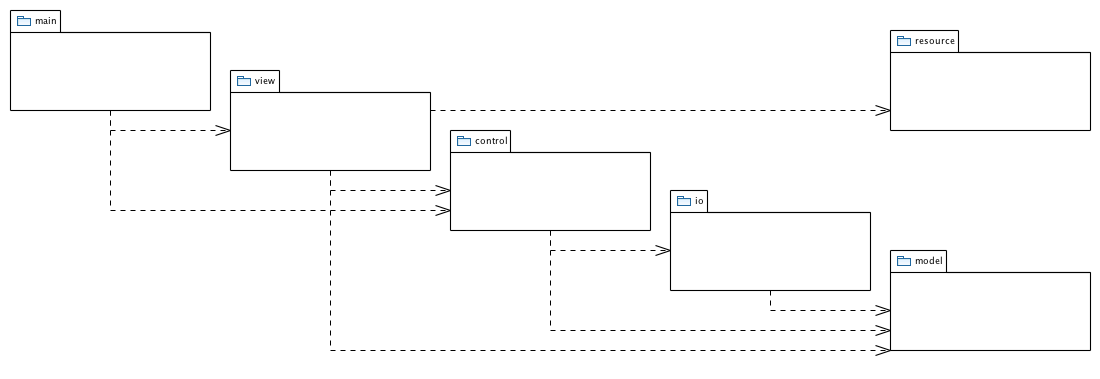
\includegraphics[width=\linewidth]{JabberPointPackageDiagram.png}
  \caption{Package diagram}
  \label{fig:packdiag}
\end{figure}


\subsection{Programming guidelines}
At the code level we improved the JabberPoint application significantly.
A list of optimisations :
\begin{itemize} 
\item Incorporate general code standards.
\item Naming conventions for variables, constants, methods, classes and packages
\item Access modifiers for constants, variables and methods 
\item Javadoc when necessary
\item Removed duplicate constants, variables, methods and code.
\end{itemize} 
We expect it would be even better if we had incorporated specialised tools to check things such as the code style, the structuring and bugs. 

\subsection{Design patterns}
\subsubsection{Model-View-Controller (MVC)}
The MVC pattern separates the model, the controller and the view.   
\begin{itemize}
\item The model manages the data, logic and rules of the application.
\item The controller accepts input and converts these to commands for model or view.
\item The view is responsible to display the information from the model to the user and respond to user actions.   
\end{itemize}
Especially removing the view dependency from the model promotes flexibility of this design pattern. This prepares for changing or adding views without changes in the model.

\subsubsection{Observer pattern}
The Observer pattern decouples the JabberPoint model from the view. This is part of the MVC pattern. The view is registered as a listener, which is notified when the model changes. In the model the class Presentation is the Observable and the Observer is the SlideViewComponent class.

\subsubsection{Factories}
The design consists of factories to have a single point for object creation for each type of object. This supports the \textit{program to interface} idiom, because the factories create the concrete implementations, while the application only depends on the abstract concepts. The factory classes are named XxxxFactory and are put in the factory package to make them recognizable.
Currently we have factories for the classes SlideItem, Slide, Presentation, Style and Theme. With the factories we provide an single way to instantiate the classes needed.

\subsubsection{Strategy pattern}
The strategy pattern facilitates the varying drawing behaviour of the slide items. The ItemDrawing interface defines the methods needed to draw slide items. The implementation of the draw function is executed according to the TextDrawing or ImageDrawing strategy. If  in the future another type of slide item is introduced, the ItemDrawing interface is implemented for the new algorithm. We looked at the composite pattern as well. SlideViewComponent has draw functionality and has multiple slide items such as text and images with draw functionality as well. The SlideViewComponent would be the composite. However, we judged this pattern as an overkill, because the structure is not a real tree. We already know where the leaves are and there is no need foreseen to interchange leaves with composites (slides in slides).

\section{Choices}
We embrace iterative development and work time-boxed. To respect the given deadline does not change our goal to deliver quality, but the application will not be perfect. This is a choice. We are convinced that we made great steps forward in the design and implementation of the JabberPoint implementation.

We redesign the application according to the \textit{Redesign guidelines} document to achieve better quality in design and implementation. This choice results in better maintainability and more flexibility. We see this as an investment in future developments that will prove prosperous in the end. The alternative was to just implement the theme functionality while retaining the bad design and implementations. We could do it even faster and much uglier, without any satisfaction to end the users, the product owners and ourselves.

Bugs are fixed. This choice refers to clear bugs that can be fixed without big risks of introducing unexpected behaviour. Quality of the application and user experience are important. The alternative of leaving all the bugs in was just no option to us.

Given the major redesign and refactoring we decided to label the application version 2.0. We could have chosen version 1.7, but we think a major upgrade, with design and functionality changes, reflects a major version better. 

The report and documentation are in English, not Dutch. English is the obvious choice as software development is often cross-border. Main reason: flexibility regarding the future developments of the product without much initial investments. Besides this, it is a good exercise for students.

Support for the current file format is continued. The application will display the test.xml file correctly as well as files that are in the wild. Customer trust and satisfaction are essential. If we dropped support then users will get stuck with presentations that can only be opened with older JabberPoint versions.
 
The file format is allowed to alter, but the implementation must be backwards compatible. This allows the introduction of new features while still supporting all presentations for all users. The alternative would be that the presentation file would not contain the theme. This could be done by not saving the theme at all or save it in another file that had to be related somehow with the presentation file. A good user experience and simplicity lead to the choice to alter the file format.

We made a choice to provide the themes with the presentation files. In this case there can be modifications to the theme and when transferring the presentation it is still possible to see the presentation as intended. We made the choice to be backward compatible. When there is no theme information in the presentation file the default theme will be used. In the application we build hard coded several themes. Normally we would have done this using an specific theme xml file which contains the different themes. However due to the time this would take to implement this we made the choice to just hard code these themes \(they are reachable using the View->Theme menu. \) In the hard coded themes we only changed the font name. We didn't implement different colours in the hard coded themes. Using the presentation file you can set this information.

The menu item \textit{Open} is implemented to let the user open a new presentation. This menu item did not provide this functionality. We assume that users appreciate this implementation. There were no specifications, but we believe the behaviour of the \textit{Open} menu item is what users expect without much discussion. It can be extended with functionality, such as for example file filters, later on.

The menu item \textit{New} is removed, because the user experience of just removing the presentation was not good. The no editing nature regarding presentations did not correspond to the creation of a new empty presentation. In the context of clear and unambiguous functionality, we decided to remove the menu item completely.

The menu item \textit{Save} was kept, because it allows a user to save a theme selection. We decided that if a user has selected a theme for a presentation then the expected behaviour of the application that it would apply that theme to the presentation automatically. The user can store the theme by choosing the menu item.

We decided to keep two switch statements because these are both clear and simple. There is a switch statement in a factory class, where occasionally switches or if statements are necessary to handle different parameter values. And there is a switch statement to handle the key that was pressed by the user. Different implementations like a strategy pattern or something else would result in more complex, thus less maintainable code. That this is a reasonable decision is apparent from the implementation of java itself, where the switch statement is used often in high profile classes such as \texttt{java.awt.event.KeyEvent}.

We decided to start with the implementation of localisation. For now it is kept simple, only supporting the en\_US locale. With this, the application has centralised labels and is prepared for other languages in the future.   

We designed the package structure according to the package-by-layer style. Generally, this style is easier to understand and more common than the package-by-feature style. If in the future a new view, like a web application, is required then we expect it to be easier to support as the view and controller classes are in well defined layers with well defined dependencies. Of course, the package-by-future style has advantages too, but we still preferred the layer style.

\section{Sourcecode}
\subsection{Startup and load presentation}
The entry point of the application is the \texttt{JabberPoint} class which is located in the main package. The main method starts with the creation of the two controller classes: \texttt{PresentationController} and \texttt{ApplicationController}. The view is created via the \texttt{SlideViewerFrame} class and the \texttt{ApplicationController} is registered as a listener to it. The view is then registered as a listener or observer to the \texttt{Presentation}. Now, the application setup is finished so is the \texttt{JabberPoint} class. The last thing to  do is calling the method \texttt{loadPresentation} of the \texttt{ApplicationController} passing the optional command line parameter.

The \texttt{ApplicationController} the delegates the creation of a \texttt{Presentation} to the \texttt{PresentationController} and the \texttt{PresentationFactory}. The method \texttt{createPresentation}  receives the optional command line parameter. The \texttt{PresentationFactory} instantiates an \texttt{Accessor} to load and return a \texttt{Presentation}. If no startup parameter was received then \texttt{DemoPresentation} is returning the \texttt{Presentation}, otherwise \texttt{XMLAccessor} will return a \texttt{Presentation} loaded from disk.

The \texttt{ApplicationController} tells the view, which implements the \texttt{PresentationObserver} interface to listen to the created \texttt{Presentation} object. Setting the current slide to 0 triggers the view to display the current \texttt{Slide} of the \texttt{Presentation}.

To facilitate testing the application comes with two XML files: 
\begin{itemize}
\item \texttt{test.xml}: the original file delivered with the assignment
\item \texttt{test-new.xml}: showcase of new functionality
\end{itemize}

\subsection{Domain classes}


\subsection{Show frame, slide and items}



\end{document}
